\title{jeffery_lim}
\documentclass[11pt, a4paper]{article}
\usepackage[utf8]{inputenc}

\usepackage{listings}
\usepackage[framed,numbered,autolinebreaks,useliterate]{mcode}

\usepackage[margin=1in]{geometry}
\usepackage{graphicx}
\usepackage{amsmath}
\usepackage{float}
\graphicspath{ {../images/} }
\setlength\parindent{0pt}

\begin{document}

\begin{center}
  \Huge ECEN4532, DSP Laboratory \\
  \huge Music Classification \\
  \huge Lab 3\\
  
  \vspace{7in}
    \huge Jeffery Lim \\
    \huge Jeffery.Lim@colorado.edu\\~\\~\\
\end{center}
\pagebreak

\tableofcontents

\pagebreak

\section{Introduction}

For the last lab concerning music, songs will finally be classified and a prediction method will be developed in order to properly determine the genres of each song. The first half of the lab is to determine a good way of calculating distance, and this will be utilized by finding KLDistances. This distance matrix will then be used in order to do classifying of genres.


\section{KLDistance}
The KL distance function takes in a two coefficient matrices and a gamma value. The one big factor is the introduction of $-\infty$. This was discovered during debugging and identical songs would cause the exponential term to go to infinity, thus making d = $-\infty$. This was fixed where $-\infty$ was replaced with 1. To calculate d, a different method was used from guidance from Professor Francois Meyer. This means the gamma value actually ranges from 10 to 100. Using the original distance calculation would only cause the distance matrix to place heavy emphasis on the diagonals, and not the actual collection of songs. 

\lstinputlisting[language=Matlab]{../KLDistance.m}

\subsection{Distance Calculation}

\subsection{Preparation}

The preparation of the mfcc and npcp distance matrix involved organizing the data in a fast and efficient method. The first part of the code calculates the mfcc and npcp matrix values for each song and saves them into a results directory. \\

The steps is as follows:
\begin{itemize}
    \item Load all songs
    \item mfcc and npcp matrix generation
    \item save mfcc and npcp to a result directory
\end{itemize}

A lot more work could be done to minimize the amount of work the code takes, such as going further and calculating $\mu$ or $\mathrm{Cov}$ as opposed to the entire mfcc and npcp matrix. For the testing of different gamma values, 120 seconds were taken from each song. 


\lstinputlisting[language=Matlab]{../workspace_a.m}


workspace\_a.m is the first step, which loads the songs and saves the mfcc and npcp matrix into a directory, which would be later reloaded. This saves a lot of time on the calculation and optimization of gamma. 

\lstinputlisting[language=Matlab]{../loadCoefficients.m}

loadCoefficients is the code to run when importing the data from the result of workspace\_a.m. Each mfcc and npcp matrix is stored into a cell array, which gets returned.

\subsection{Computing Distance}

\lstinputlisting[language=Matlab]{../computeDistance.m}

The computeDistance function takes the $\gamma$, and both mfcc and npcp matrix, and analyzes the KL distance between all songs.

\subsection{Gamma Optimization}

\lstinputlisting[language=Matlab]{../workspace_b.m}

Each $\gamma$ value was evaluated from 10 to 100 in increments of 10, as seen in workspace\_b.m. Initially, the graphs were compared visually, but more analysis is needed in order to determine the best $\gamma$ value. Instead of analyzing each gamma value, the analysis will be done once the best gamma value is chosen.

\pagebreak

\begin{figure}[H]
\hspace*{-2cm}    
    \centering
    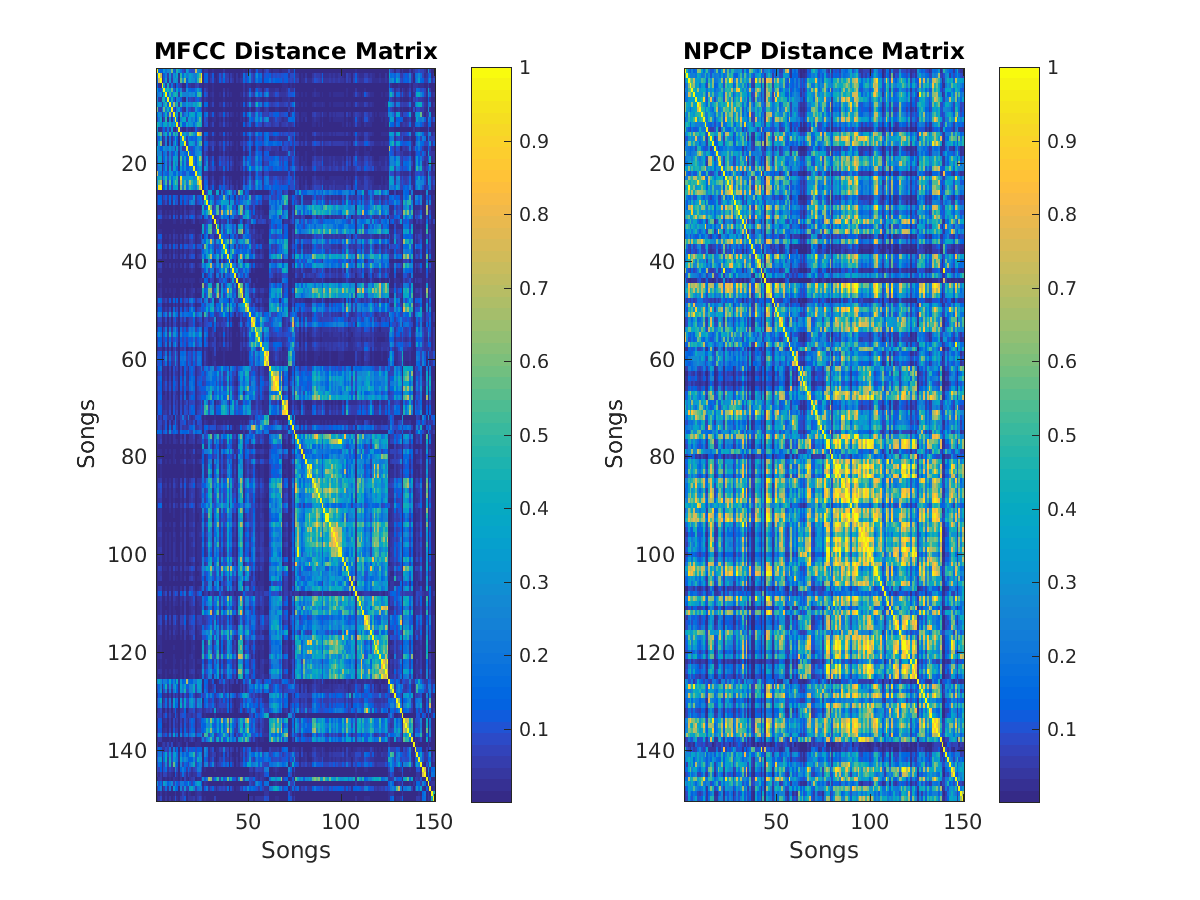
\includegraphics[width=1.25\textwidth]{gamma10.png}
    \caption{$\gamma = 10$}
\end{figure}

\begin{figure}[H]
\hspace*{-2cm}    
    \centering
    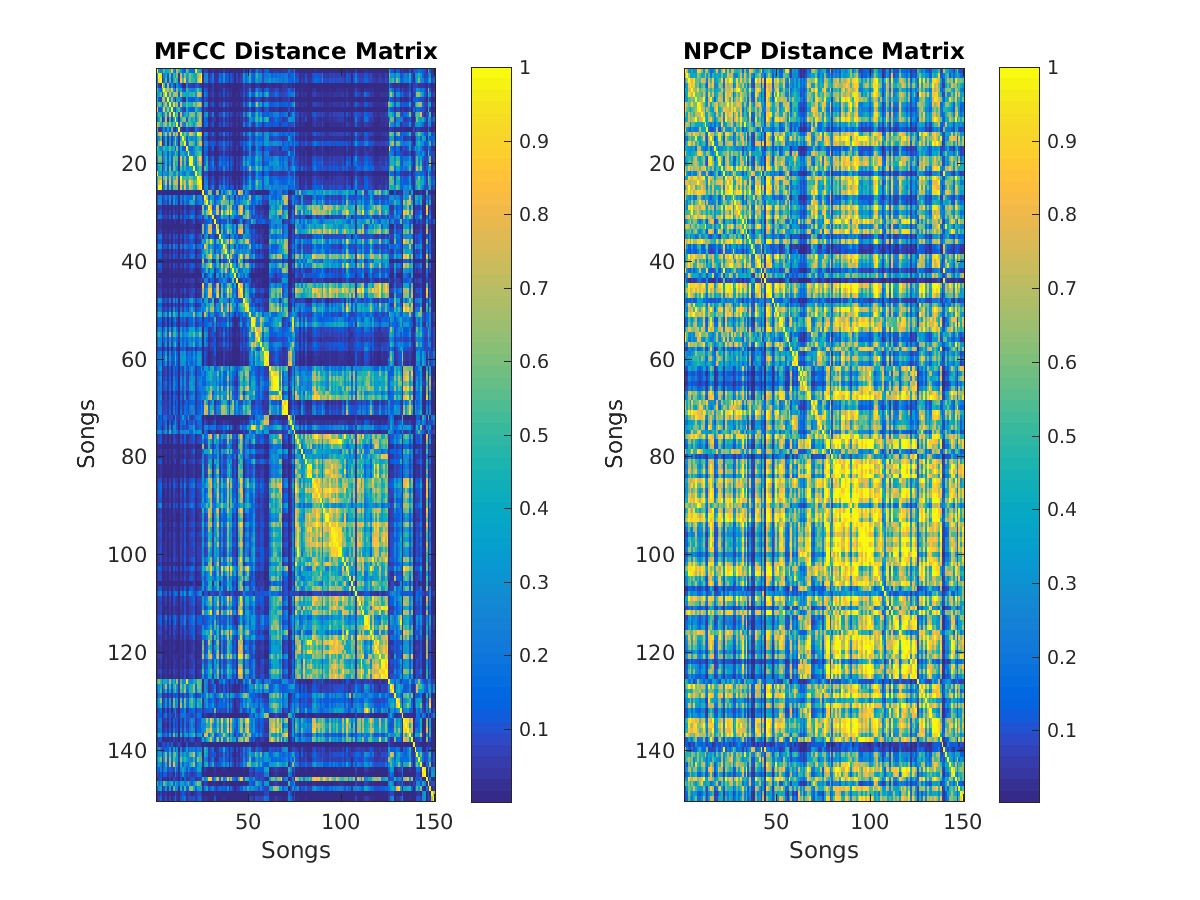
\includegraphics[width=1.25\textwidth]{gamma20.png}
    \caption{$\gamma = 20$}
\end{figure}

\begin{figure}[H]
\hspace*{-2cm}    
    \centering
    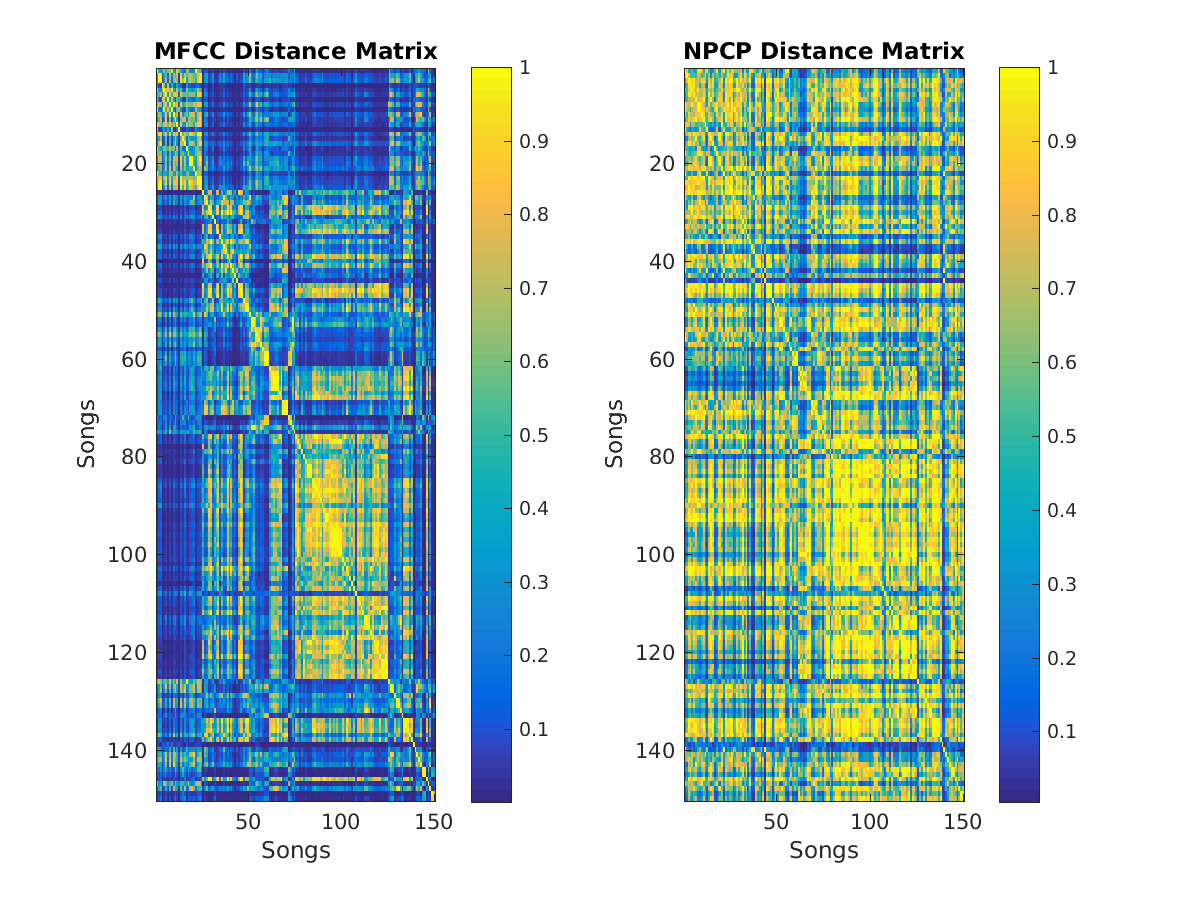
\includegraphics[width=1.25\textwidth]{gamma30.png}
    \caption{$\gamma = 30$}
\end{figure}

\begin{figure}[H]
\hspace*{-2cm}    
    \centering
    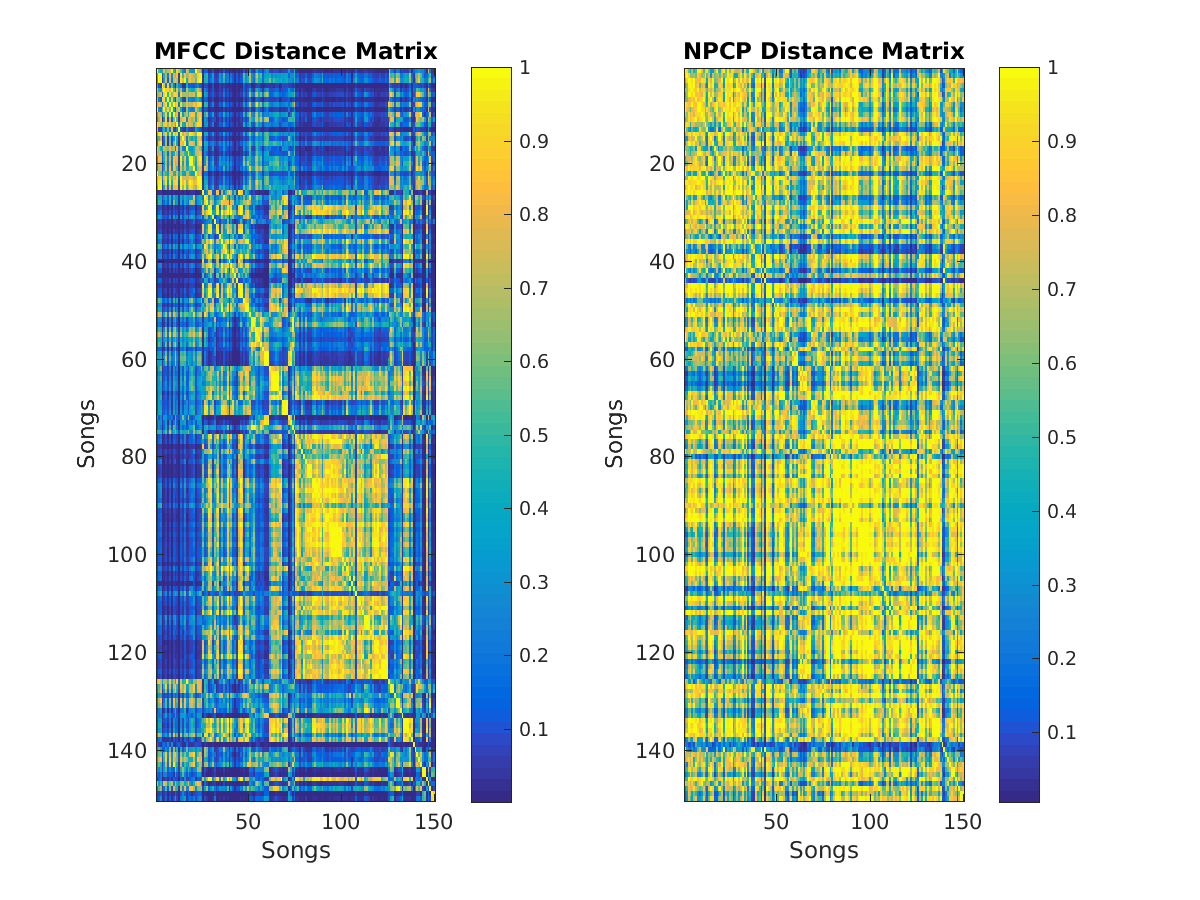
\includegraphics[width=1.25\textwidth]{gamma40.png}
    \caption{$\gamma = 40$}
\end{figure}


\begin{figure}[H]
\hspace*{-2cm}    
    \centering
    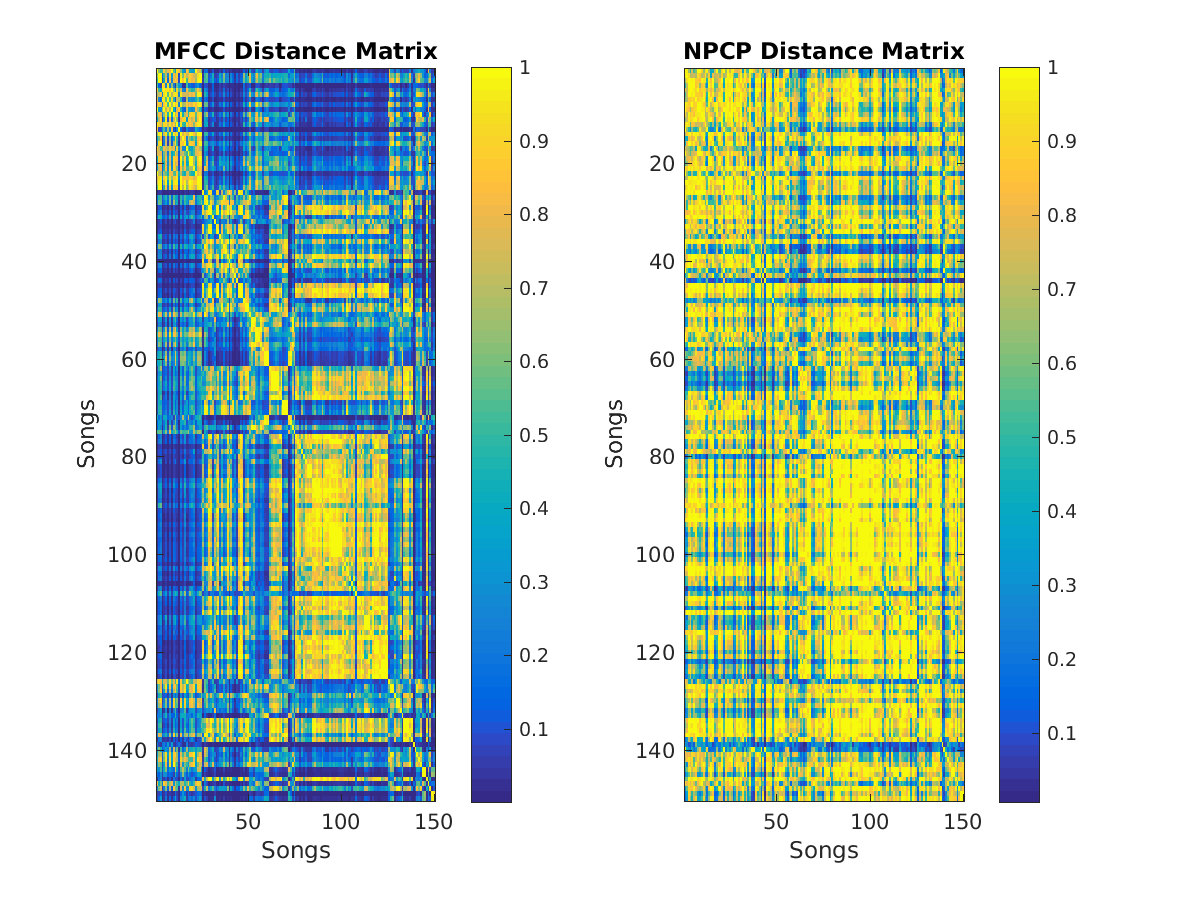
\includegraphics[width=1.25\textwidth]{gamma50.png}
    \caption{$\gamma = 50$}
\end{figure}

\begin{figure}[H]
\hspace*{-2cm}    
    \centering
    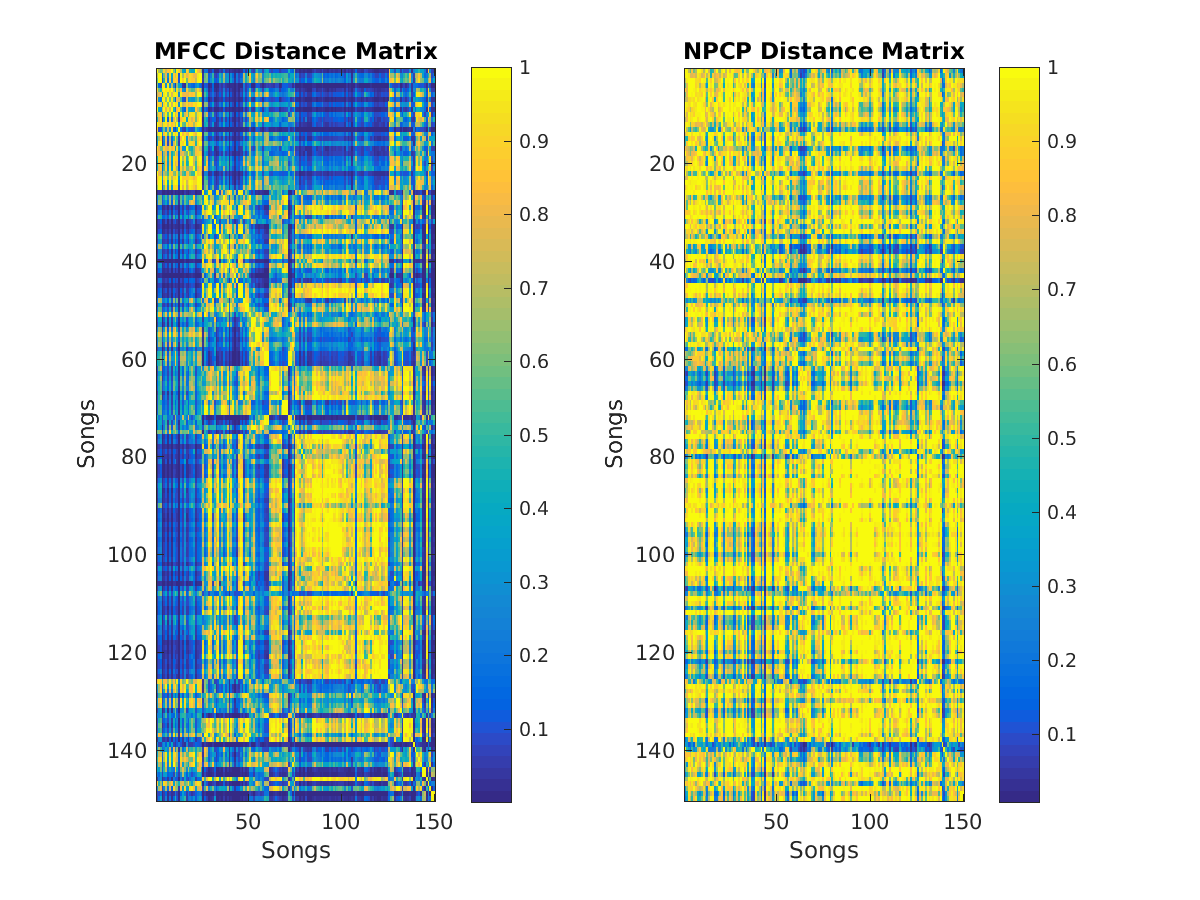
\includegraphics[width=1.25\textwidth]{gamma60.png}
    \caption{$\gamma = 60$}
\end{figure}

\begin{figure}[H]
\hspace*{-2cm}    
    \centering
    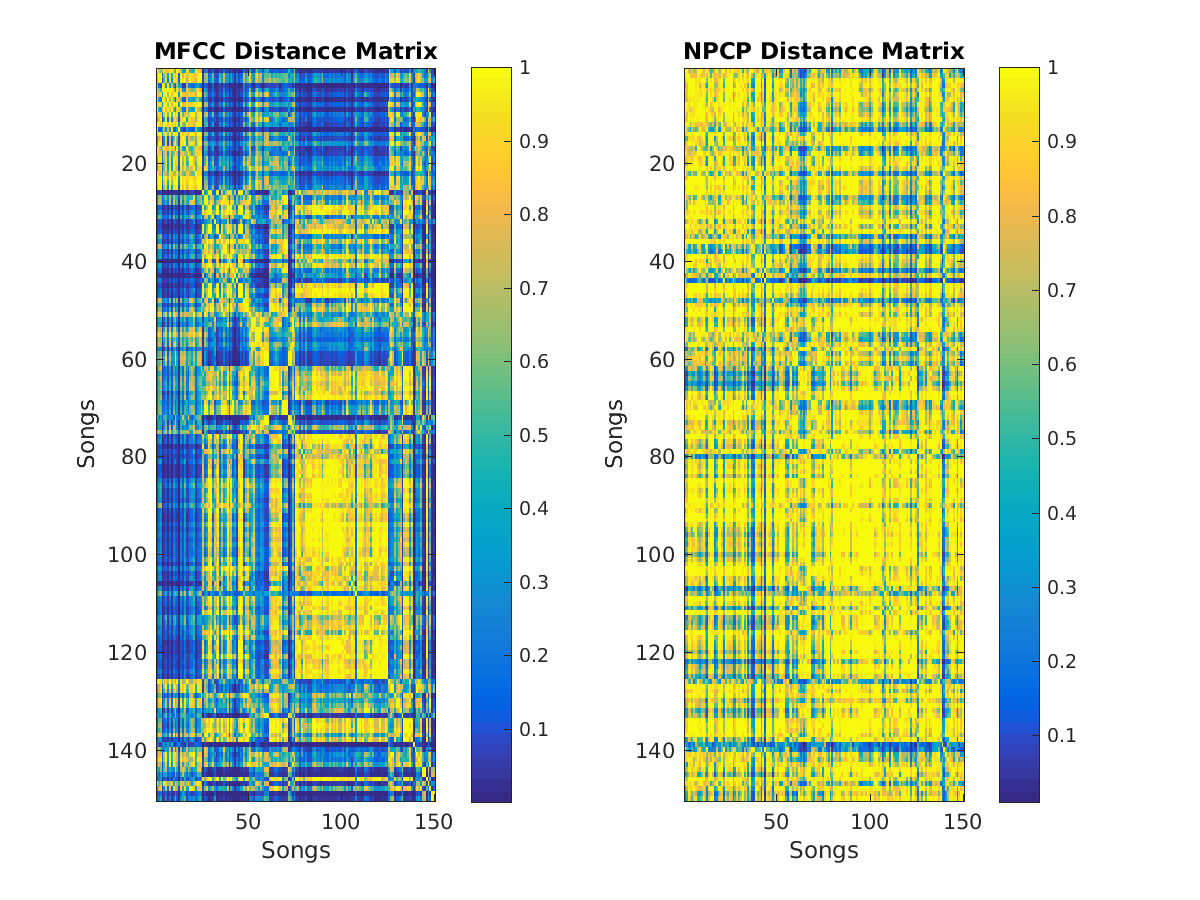
\includegraphics[width=1.25\textwidth]{gamma70.png}
    \caption{$\gamma = 70$}
\end{figure}

\begin{figure}[H]
\hspace*{-2cm}    
    \centering
    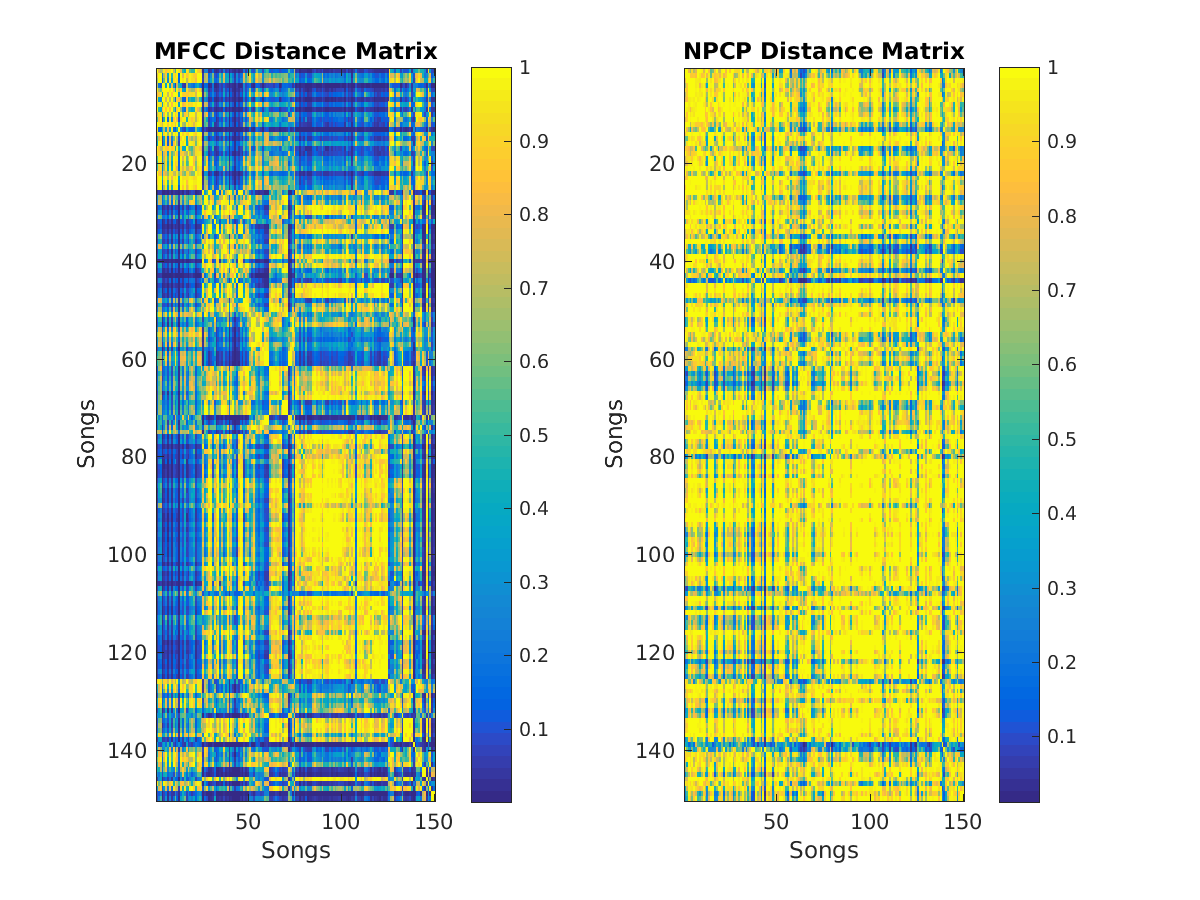
\includegraphics[width=1.25\textwidth]{gamma80.png}
    \caption{$\gamma = 80$}
\end{figure}


\begin{figure}[H]
\hspace*{-2cm}    
    \centering
    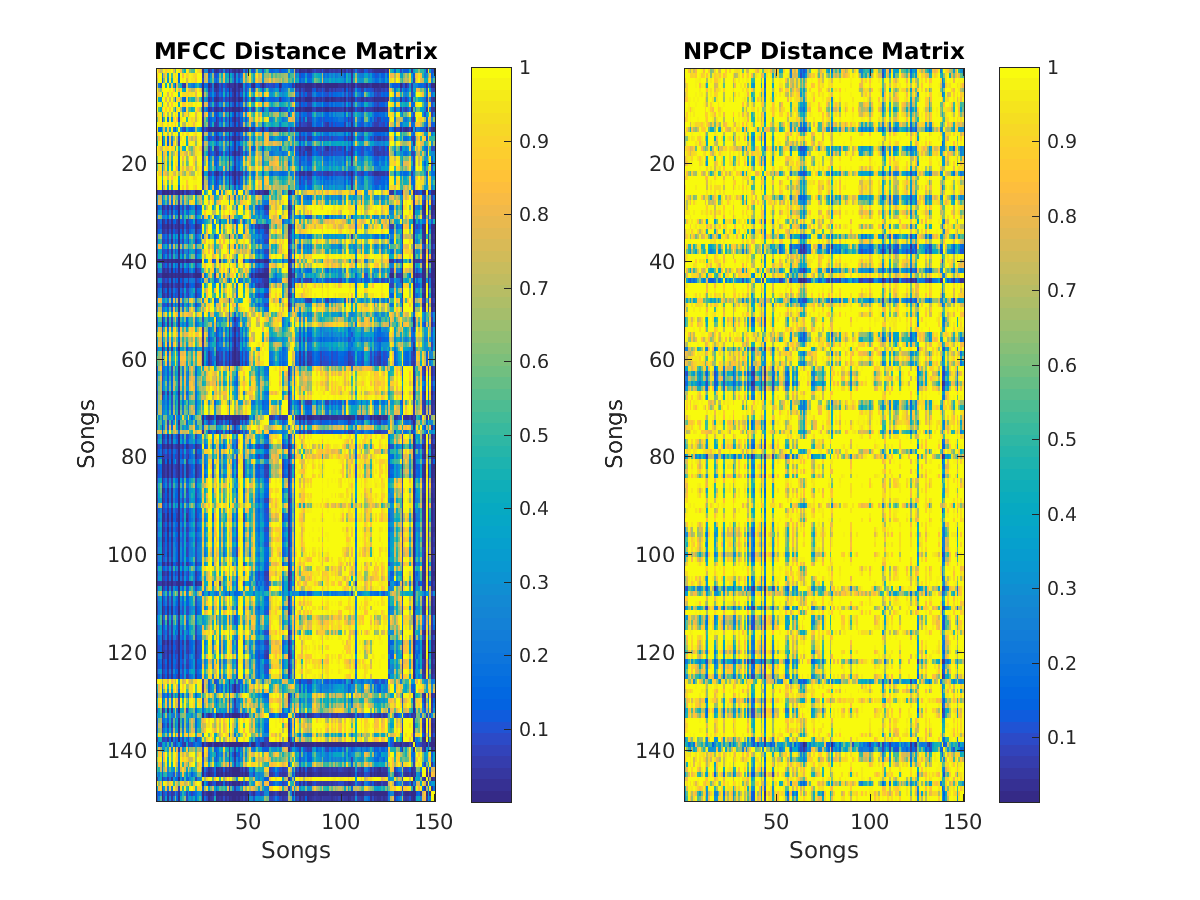
\includegraphics[width=1.25\textwidth]{gamma90.png}
    \caption{$\gamma = 90$}
\end{figure}

\begin{figure}[H]
\hspace*{-2cm}    
    \centering
    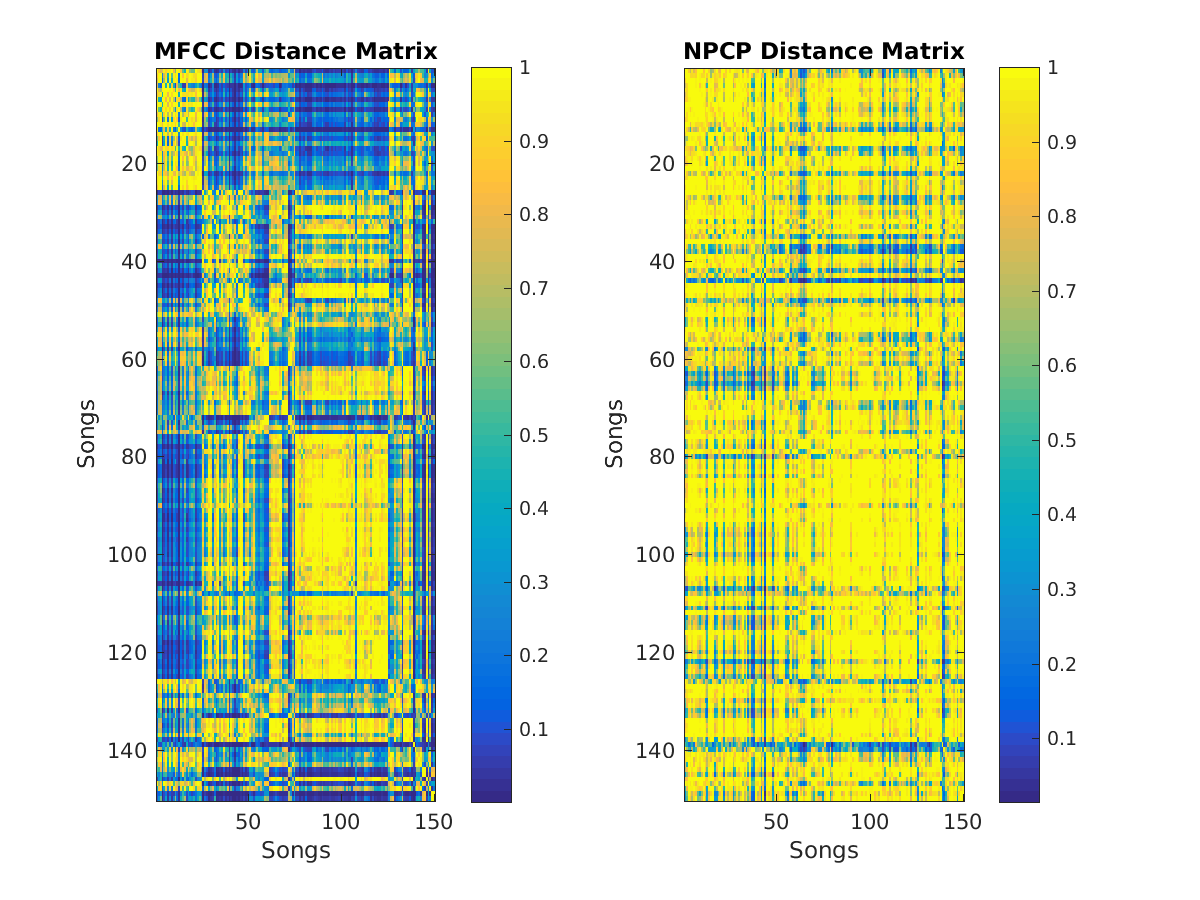
\includegraphics[width=1.25\textwidth]{gamma100.png}
    \caption{$\gamma = 100$}
\end{figure}

Overall, increasing the gamma values causes the magnitude of the overall distance matrix to increase. It helps differentiate the same genre from the others. Another thing to note is that the NPCP distance matrix is not as clear cut as the mfcc matrix is. As a result, it is expected to see that the average values will be just as obvious. \\

More specifically, throughout all the different values of $\gamma$, the classical music is very well defined within its region. There are some large values when comparing world, but considering world is a mixture of all genres, it is expected to see world have a lot of influence. \\

Punk and Rock, around songs 80 to 120, share a lot of similarities, as expected, considering the two genres are usually composed of the same instruments and somewhat similar styles. Its expected that these two genres may be difficult to differentiate from each other. \\


\pagebreak
\section{Averages}

workspace\_b.m covers the averaging of each genre. It simply goes through each genre and averages the genre compared to others. Overall, when comparing the mfcc and the npcp distances, it is clear that the mfcc has a more distinct differentiation between the songs. It is important to note that the average of same genres is no longer 1. \\


\begin{figure}[H]
\hspace*{-2cm}    
    \centering
    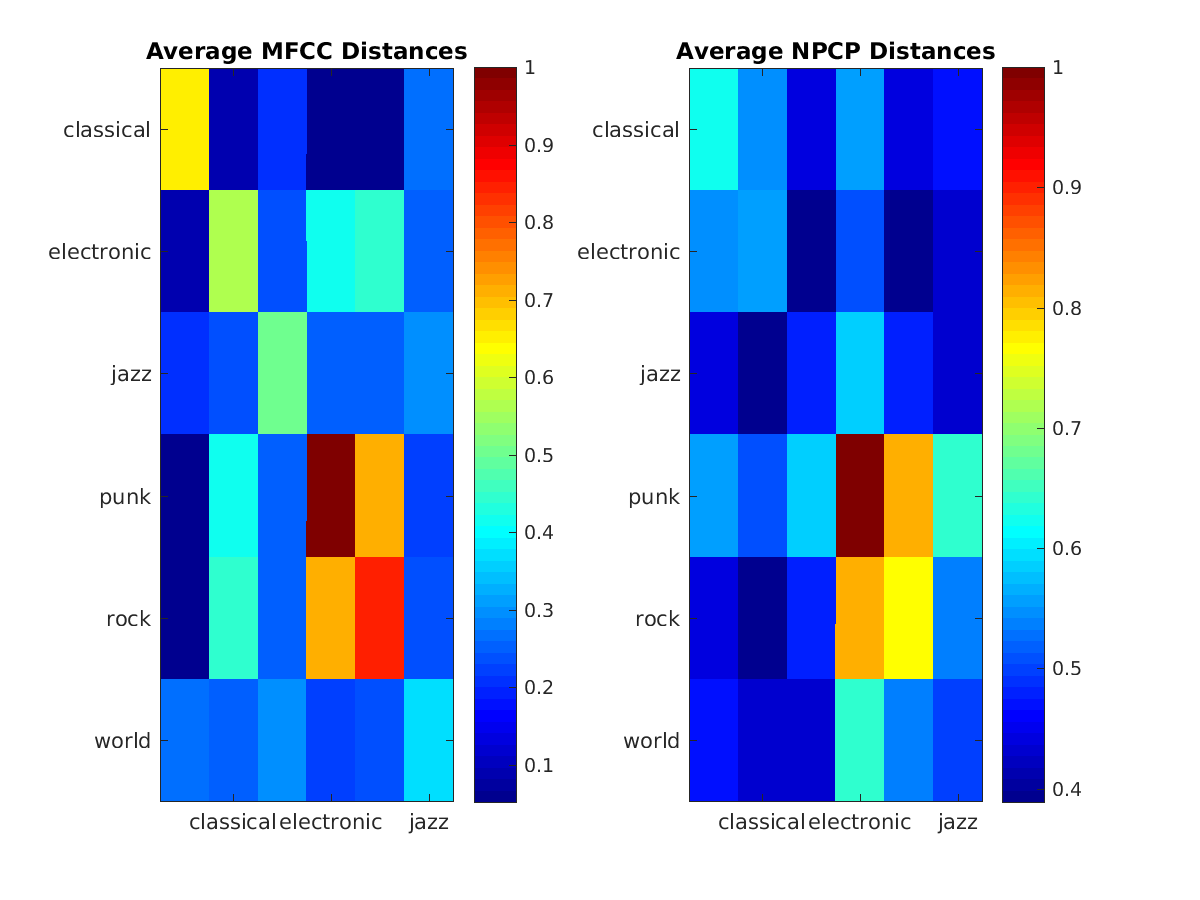
\includegraphics[width=1.25\textwidth]{average10.png}
    \caption{$\gamma = 10$}
\end{figure}

\begin{figure}[H]
\hspace*{-2cm}    
    \centering
    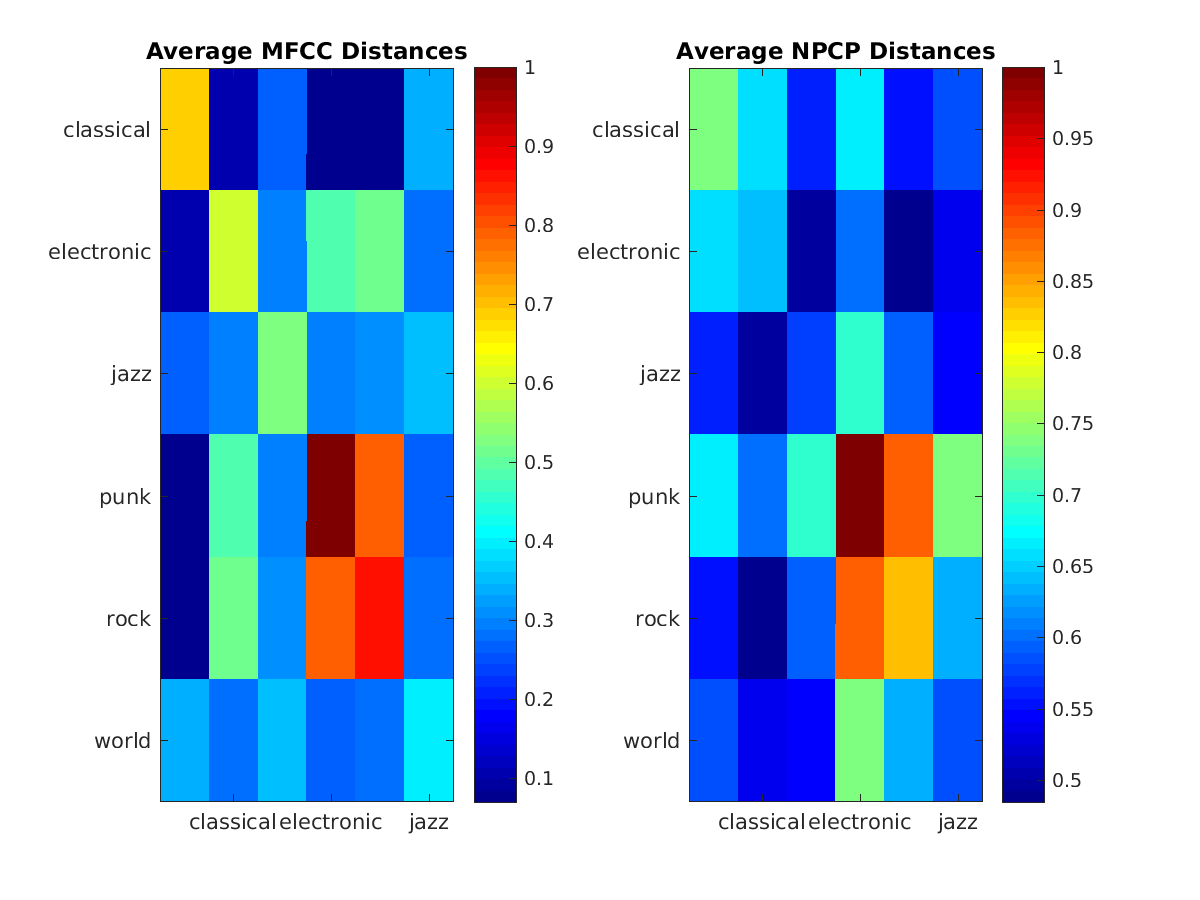
\includegraphics[width=1.25\textwidth]{average20.png}
    \caption{$\gamma = 20$}
\end{figure}

\begin{figure}[H]
\hspace*{-2cm}    
    \centering
    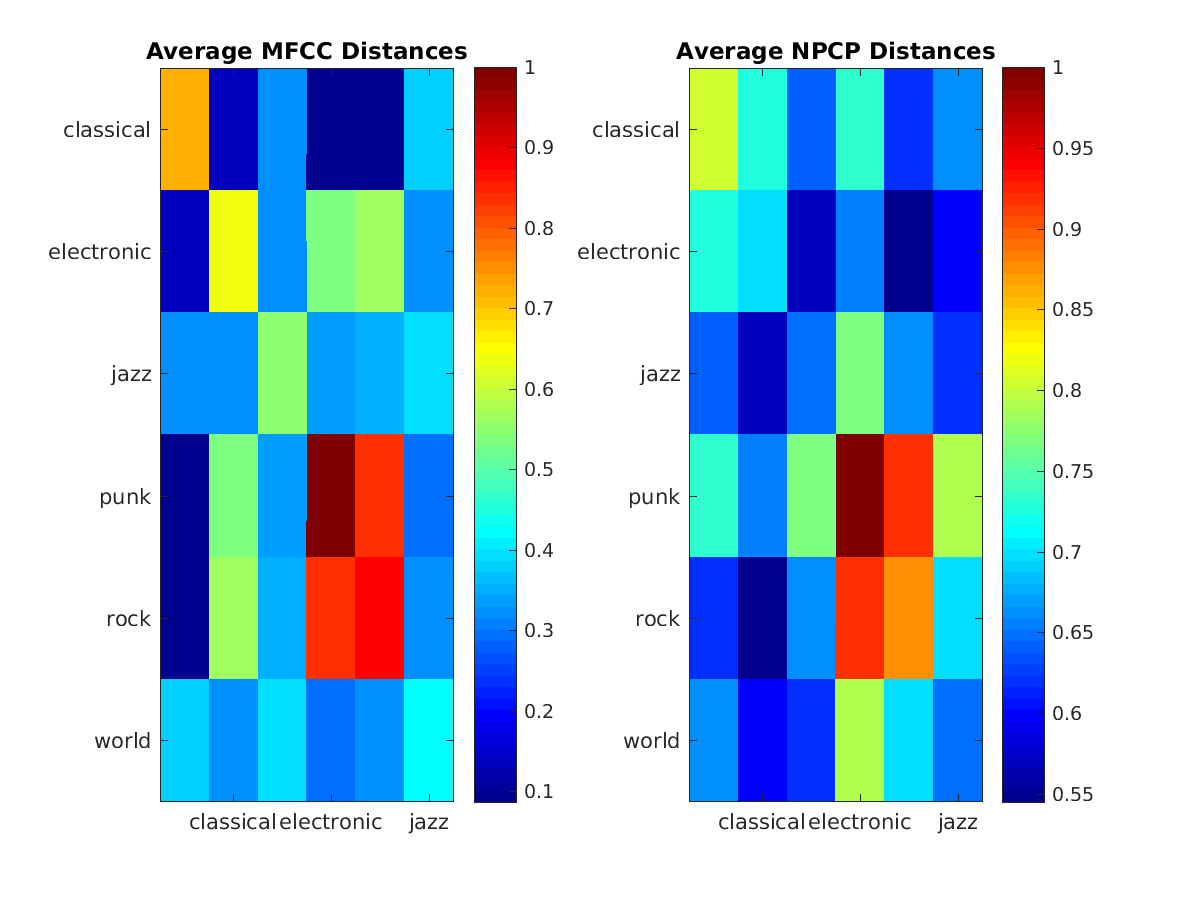
\includegraphics[width=1.25\textwidth]{average30.png}
    \caption{$\gamma = 30$}
\end{figure}

\begin{figure}[H]
\hspace*{-2cm}    
    \centering
    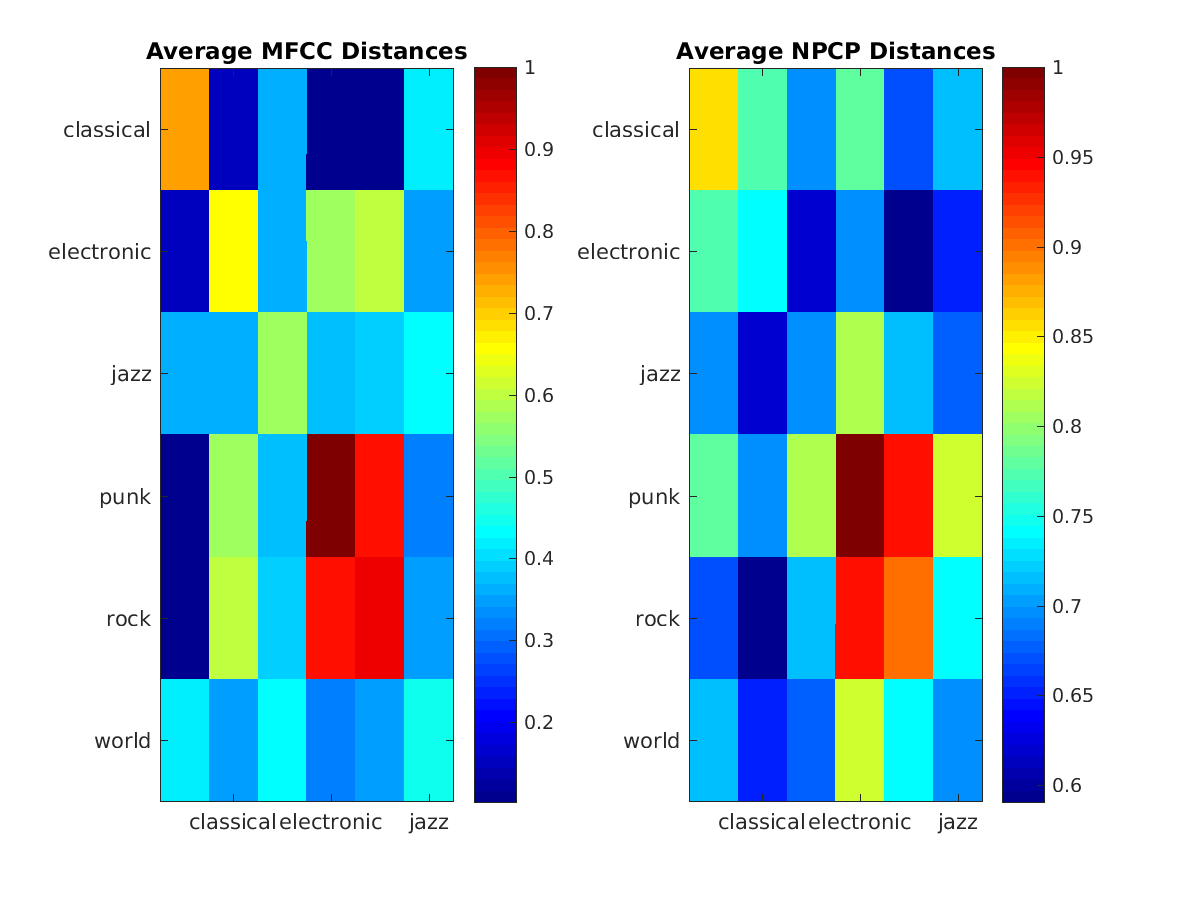
\includegraphics[width=1.25\textwidth]{average40.png}
    \caption{$\gamma = 40$}
\end{figure}


\begin{figure}[H]
\hspace*{-2cm}    
    \centering
    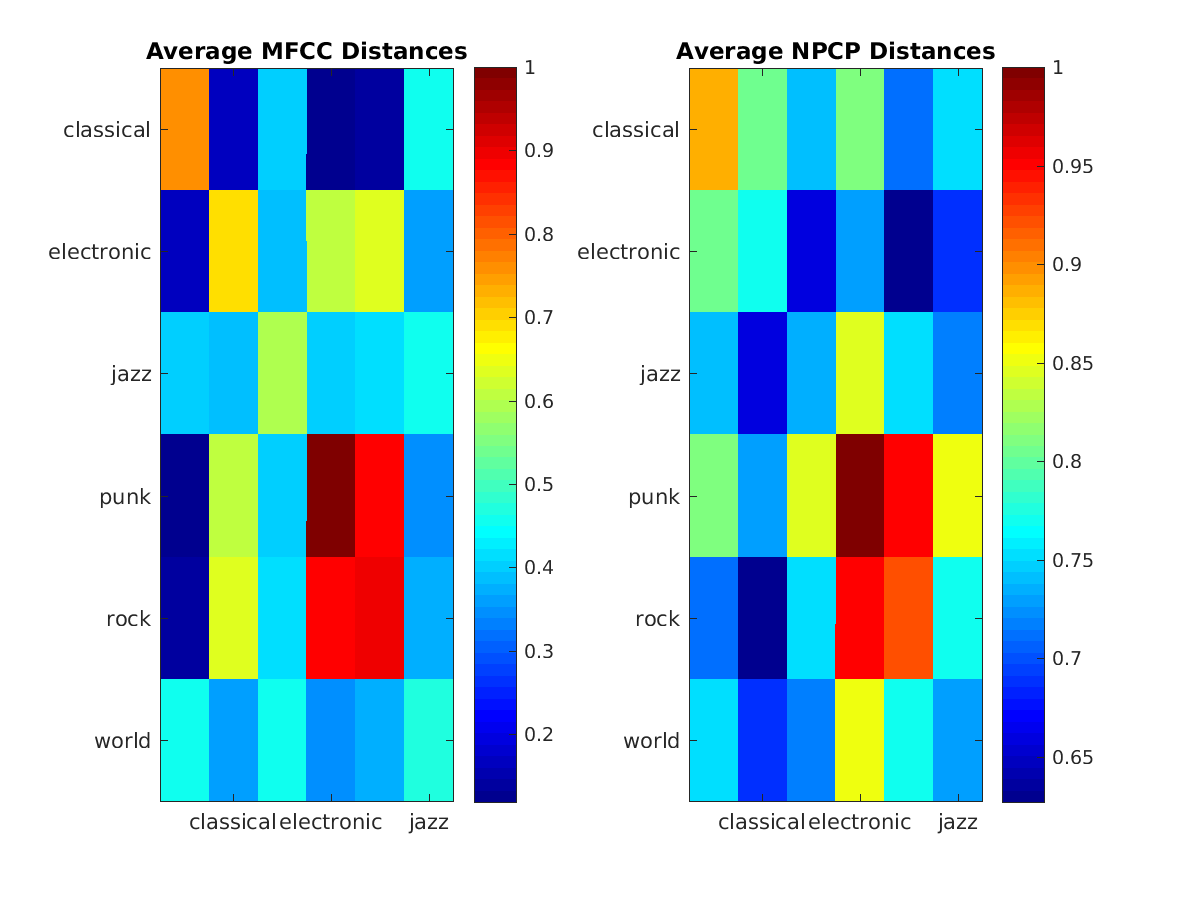
\includegraphics[width=1.25\textwidth]{average50.png}
    \caption{$\gamma = 50$}
\end{figure}

\begin{figure}[H]
\hspace*{-2cm}    
    \centering
    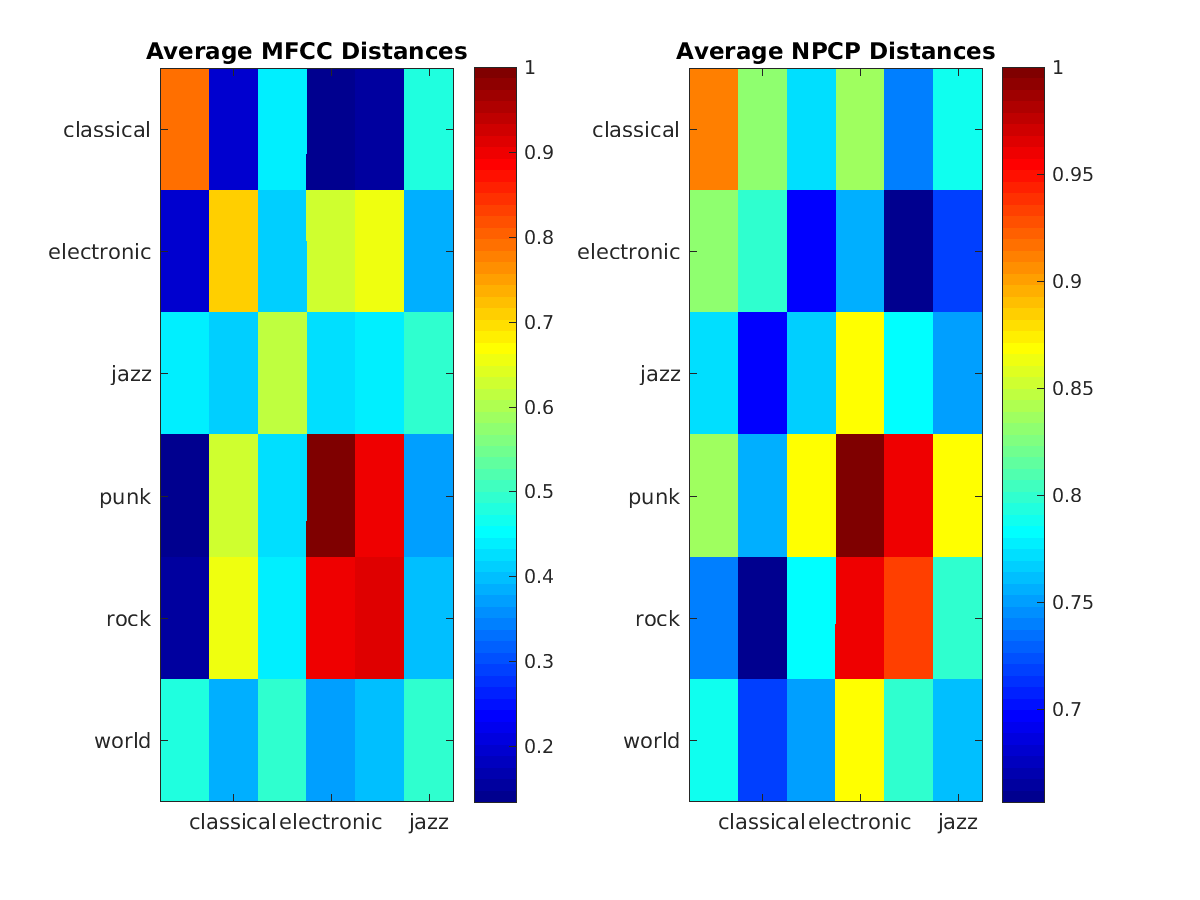
\includegraphics[width=1.25\textwidth]{average60.png}
    \caption{$\gamma = 60$}
\end{figure}

\begin{figure}[H]
\hspace*{-2cm}    
    \centering
    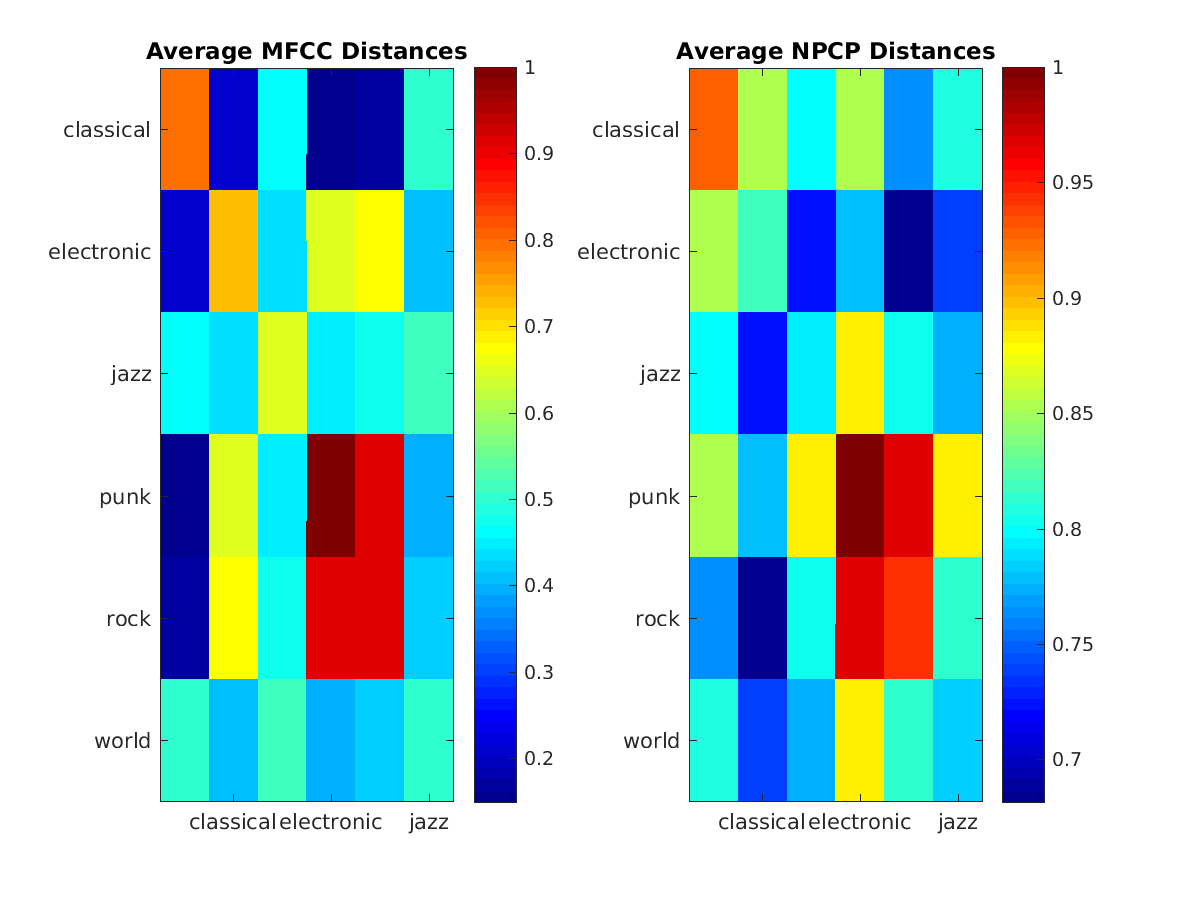
\includegraphics[width=1.25\textwidth]{average70.png}
    \caption{$\gamma = 70$}
\end{figure}

\begin{figure}[H]
\hspace*{-2cm}    
    \centering
    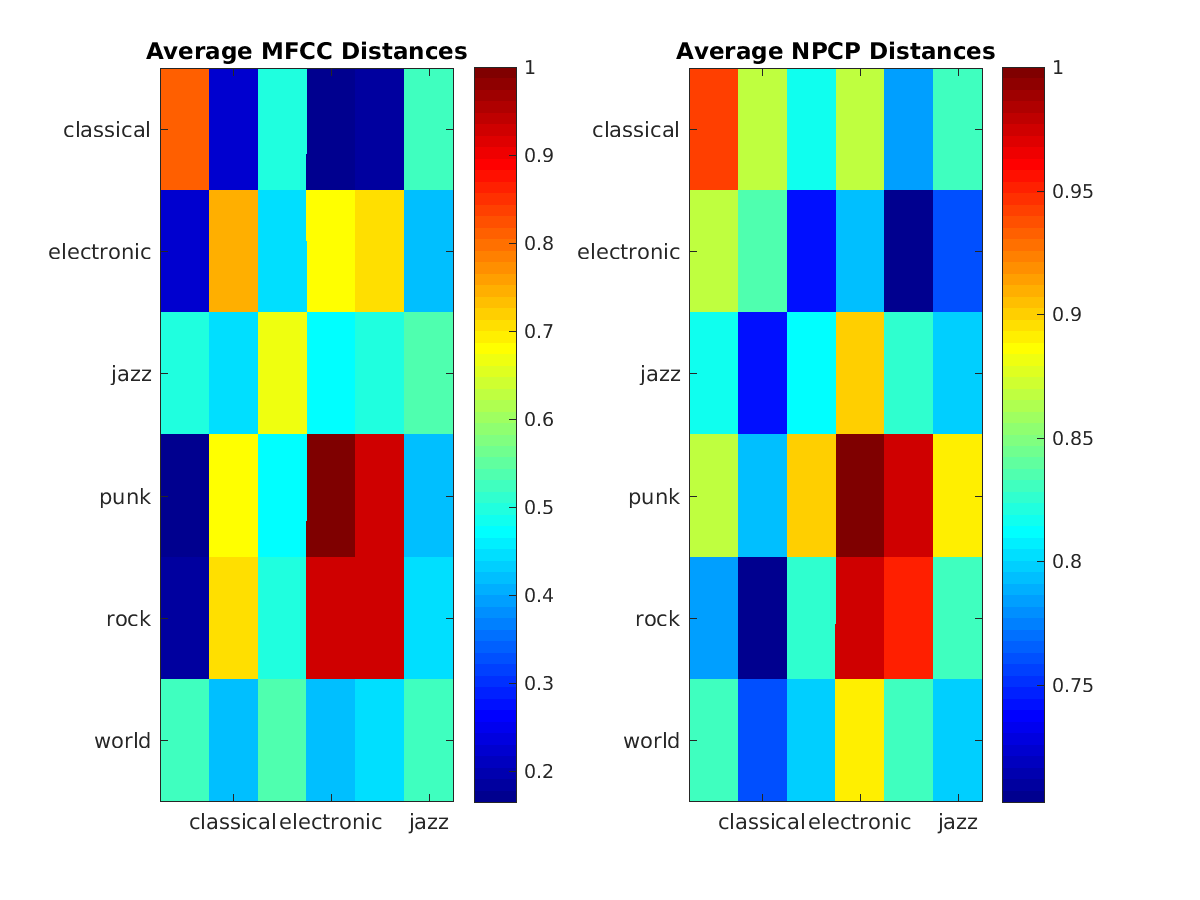
\includegraphics[width=1.25\textwidth]{average80.png}
    \caption{$\gamma = 80$}
\end{figure}


\begin{figure}[H]
\hspace*{-2cm}    
    \centering
    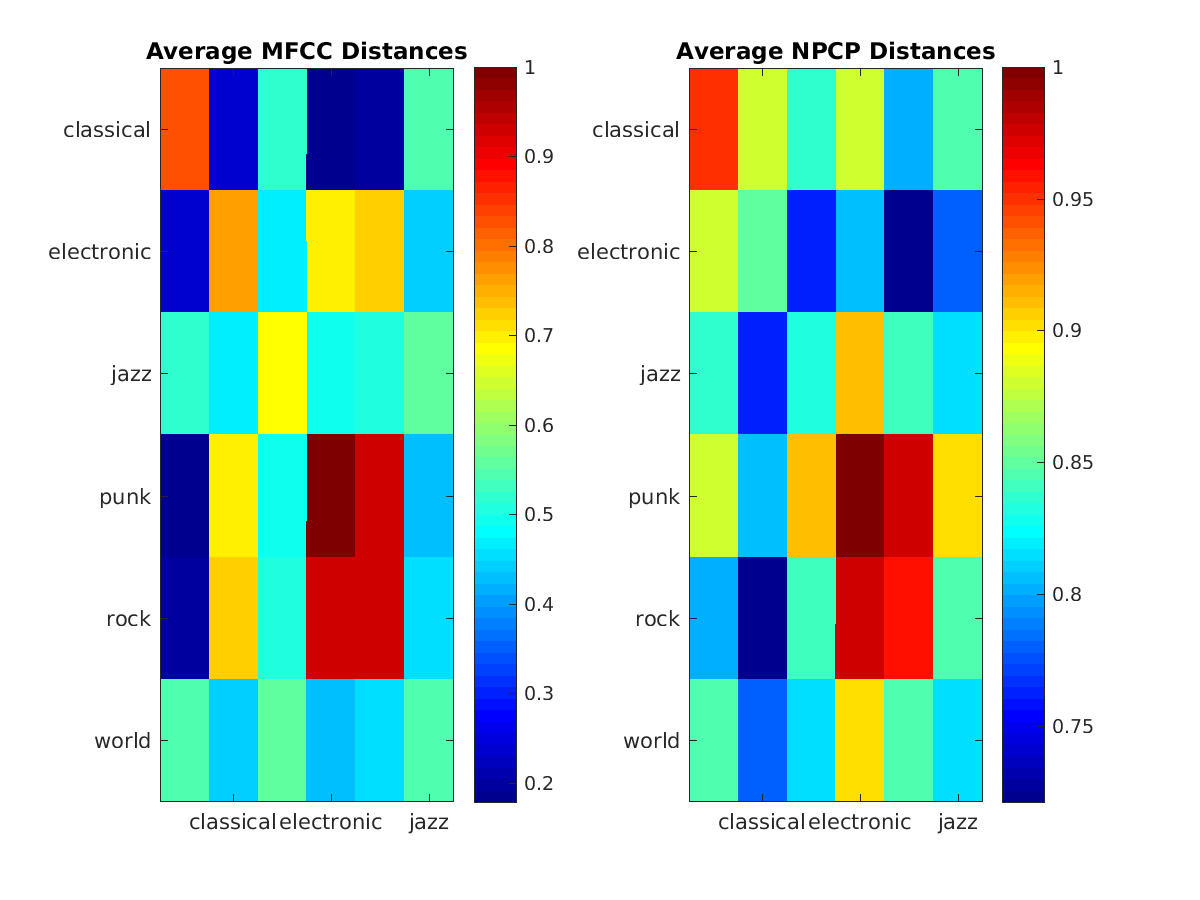
\includegraphics[width=1.25\textwidth]{average90.png}
    \caption{$\gamma = 90$}
\end{figure}

\begin{figure}[H]
\hspace*{-2cm}    
    \centering
    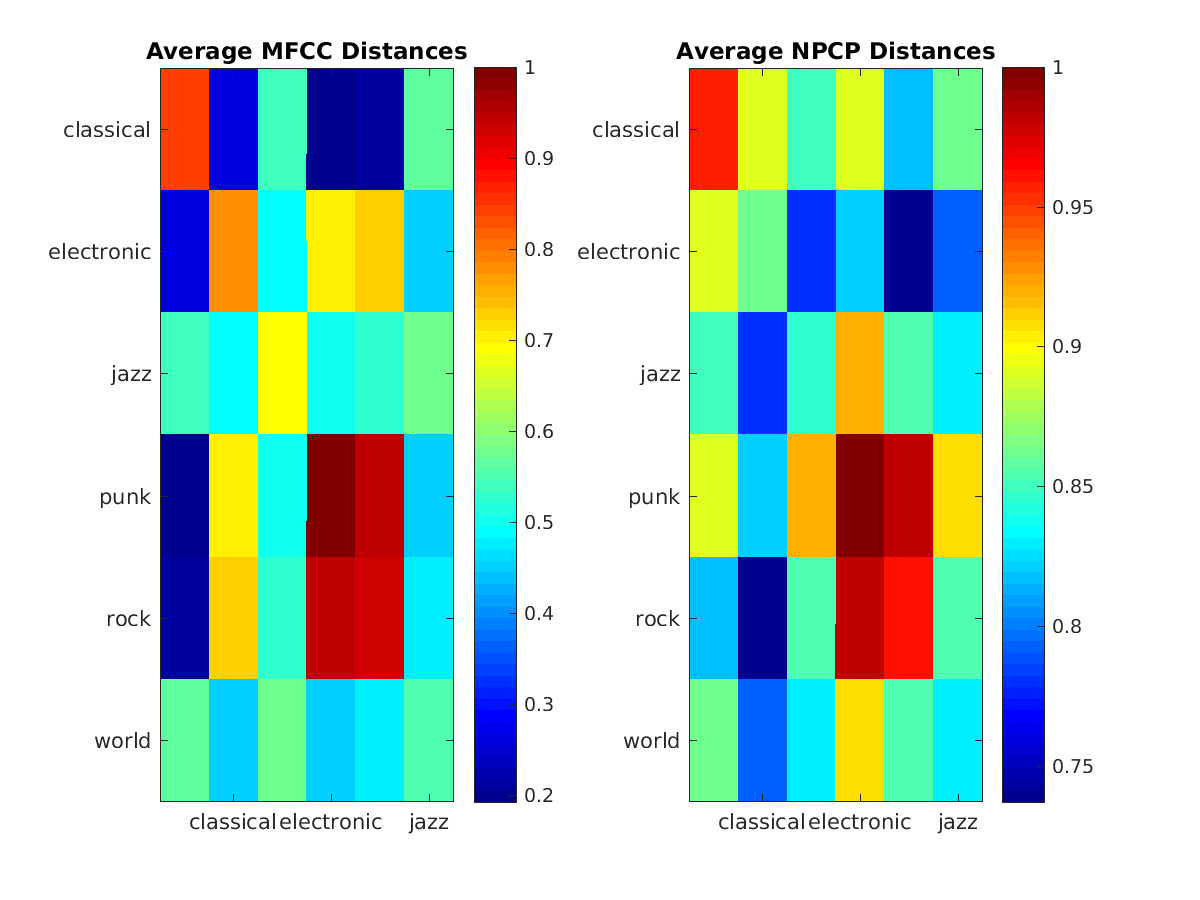
\includegraphics[width=1.25\textwidth]{average100.png}
    \caption{$\gamma = 100$}
\end{figure}


It is not efficient to determine the best $\gamma$ value using eyes, so the maximum distance value, always when classifying a genre with itself, is compared to the second maximum distance. The difference was stored into a matrix with the following results. The second maximum distance is picked because the classification needs to be sensitive and needs to minimize the difference between the largest value and the second largest. Each row represents the genre, and each column represents the $\gamma$ value, with increments of 10. \\

For the mfcc:

$\left(\begin{array}{cccccccccc} 0.148 & 0.203 & 0.236 & 0.256 & 0.268 & 0.275 & 0.279 & 0.28 & 0.28 & 0.279\\ 0.0437 & 0.0427 & 0.0406 & 0.0387 & 0.0374 & 0.0365 & 0.036 & 0.0357 & 0.0356 & 0.0355\\ 0.0614 & 0.0616 & 0.0589 & 0.0566 & 0.0552 & 0.0546 & 0.0546 & 0.055 & 0.0557 & 0.0565\\ 0.131 & 0.138 & 0.128 & 0.115 & 0.102 & 0.0918 & 0.0829 & 0.0756 & 0.0696 & 0.0646\\ 0.0478 & 0.0346 & 0.0214 & 0.0109 & 0.00288 & 0.00319 & 0.0078 & 0.0113 & 0.0141 & 0.0162\\ 0.0432 & 0.0469 & 0.047 & 0.046 & 0.0447 & 0.043 & 0.0411 & 0.038 & 0.0352 & 0.0325 \end{array}\right)$ \\

Initially looking at classical, or the first row, it is evident that the lowest difference is at $\gamma$ = 10, or the first column. As one increase the $\gamma$ value, it is increasing the difference values, however, this is a unique characteristic of classical. When looking at electronic right below it, the lowest value is actually produced when $\gamma$ = 100, but once again, it is different for Jazz with $\gamma$ = 60 or 70 being the most optimal. \\

For the npcp:

$\left(\begin{array}{cccccccccc} 0.0232 & 0.0133 & 0.00923 & 0.00812 & 0.00842 & 0.00931 & 0.0104 & 0.0115 & 0.0124 & 0.0132\\ 0.00412 & 0.00773 & 0.0158 & 0.0227 & 0.0283 & 0.0328 & 0.0365 & 0.0395 & 0.0419 & 0.0429\\ 0.0371 & 0.0772 & 0.0988 & 0.11 & 0.114 & 0.11 & 0.104 & 0.099 & 0.0935 & 0.0882\\ 0.243 & 0.235 & 0.199 & 0.165 & 0.137 & 0.114 & 0.0952 & 0.0803 & 0.0683 & 0.0585\\ 0.0273 & 0.0576 & 0.0712 & 0.0767 & 0.078 & 0.077 & 0.0748 & 0.0718 & 0.0686 & 0.0652\\ 0.0499 & 0.0691 & 0.0759 & 0.0772 & 0.0761 & 0.0738 & 0.0709 & 0.0678 & 0.0646 & 0.0614 \end{array}\right)$\\

Once again, it is not as clear which $\gamma$ value is efficient. Overall, they are not necessarily consistent. As a result, the average of each column is calculated and the largest average is used because the larger average represents a larger difference. \\

For mfcc, the value is $\gamma$ = 30, with the average difference being 0.0886.\\
For npcp, the value is $\gamma$ = 30, with the average difference being 0.0784.\\

This value of $\gamma$ will be used for the rest of the lab. \\


\subsection{Analysis}

\begin{figure}[H]
\hspace*{-2cm}    
    \centering
    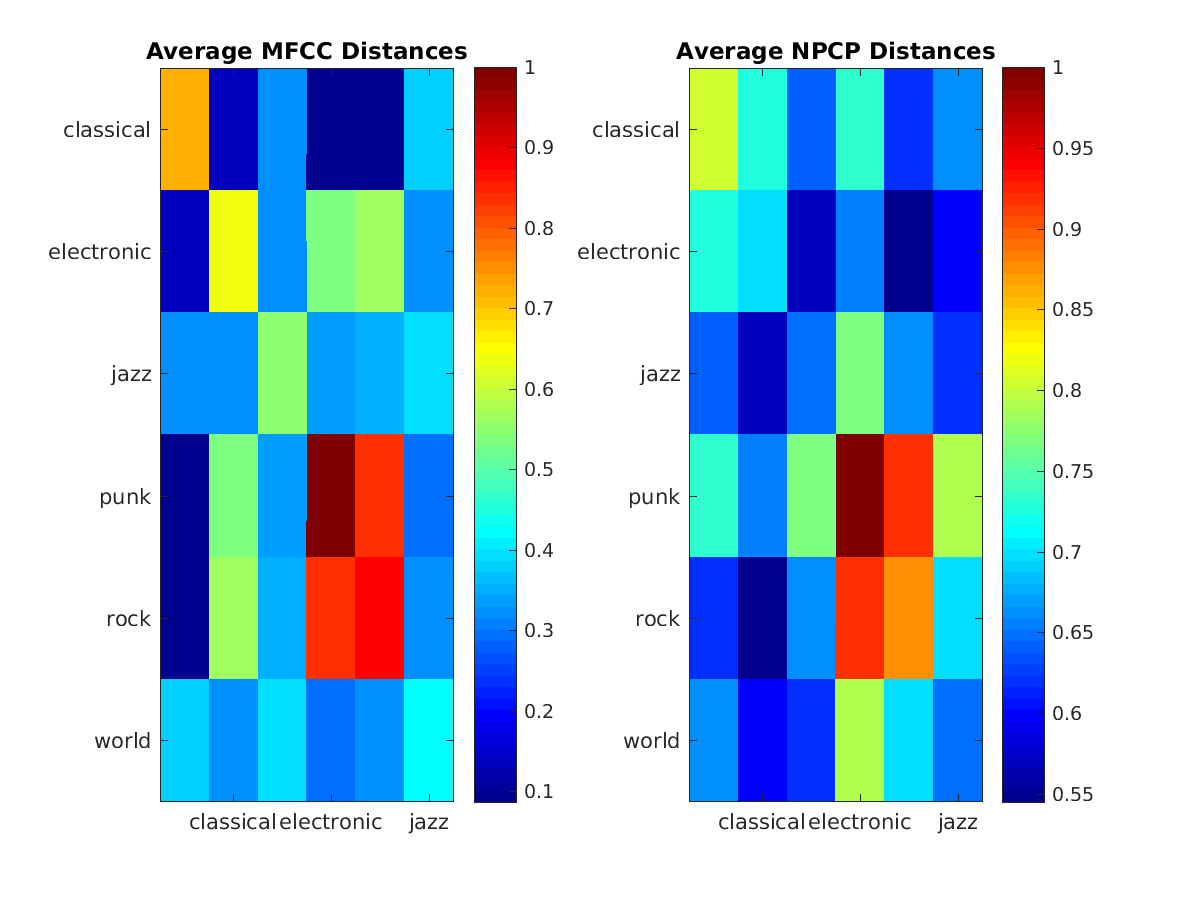
\includegraphics[width=1.25\textwidth]{average30.png}
    \caption{$\gamma = 30$}
\end{figure}

Its very interesting to note that both values point to the same gamma value to be the most efficient value to be used, but the mfcc has a larger average difference than npcp, and with this, the value of the most efficient $\gamma$ is 30. The mfcc values also give a better average distance than the npcp values as evident in the magnitudes of the diagonal in comparison to the other genres. In the npcp values, it is evident there are several misclassification such as jazz and world. \\

In the figure, the average mfcc distance shows that for classical music, it is very obvious when a song is classical. However, for songs like jazz and world, it is very difficult to differentiate between the songs. Similar genres, like punk and rock are very similar, and thus those square are very large in value.\\

Electronic is another story as it is seen that it is very similar to punk and rock. This is another problematic genre. \\

Overall, classical, jazz, and punk will have the best prediction due to the large distances between itself and the other songs. \\

Rock, world, jazz, and possibly electronic will have issues for prediction. Rock might have a lot of misclassification to punk, and world is not necessarily that different from any of the other genres.

\subsection{Histogram}
\begin{figure}[H]
\hspace*{-2cm}    
    \centering
    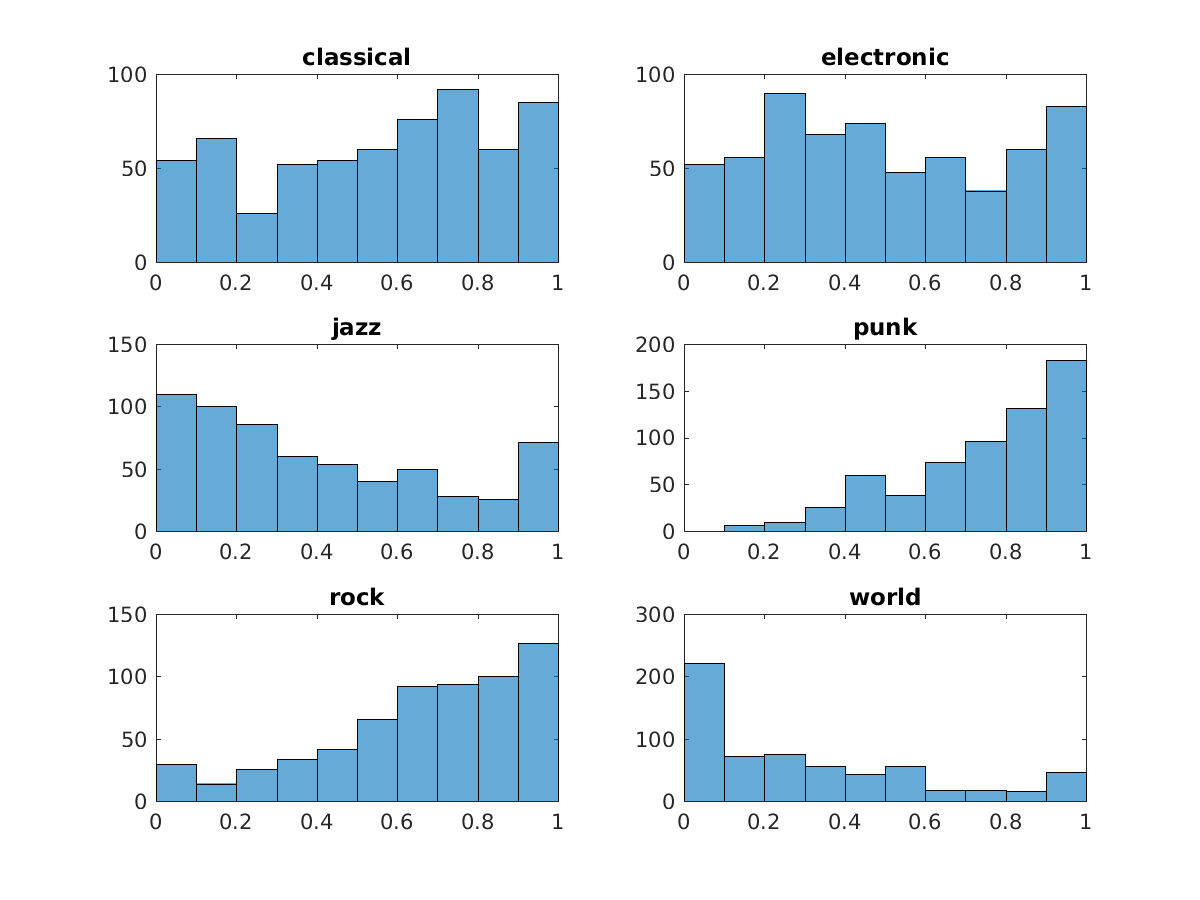
\includegraphics[width=1.25\textwidth]{histogram.png}
    \caption{Histogram of the Distances}
\end{figure}

The histogram demonstrates the spread of distances. As evident in world histogram, it is very hard to classify world as most of the histogram is very low. Punk and rock are expected to have high recognizability since they have very large values at 1. Jazz will be difficult, but not as difficult as world, and electronic and classical will be fairly simple to classify. This histogram is essentially a prediction of what the classifier should be able to predict. 

\subsection{Song Length}

For the next section, the song length is differed and the resulting averages are analyzed. The songs are analyzed at 30, 60, 120, and 240 seconds. The code used is similar to workspace\_b.m. The code is to run workspace\_a.m with the different song lengths, and then run workspace\_b.m to generate new average plots. 


\begin{figure}[H]
\hspace*{-2cm}    
    \centering
    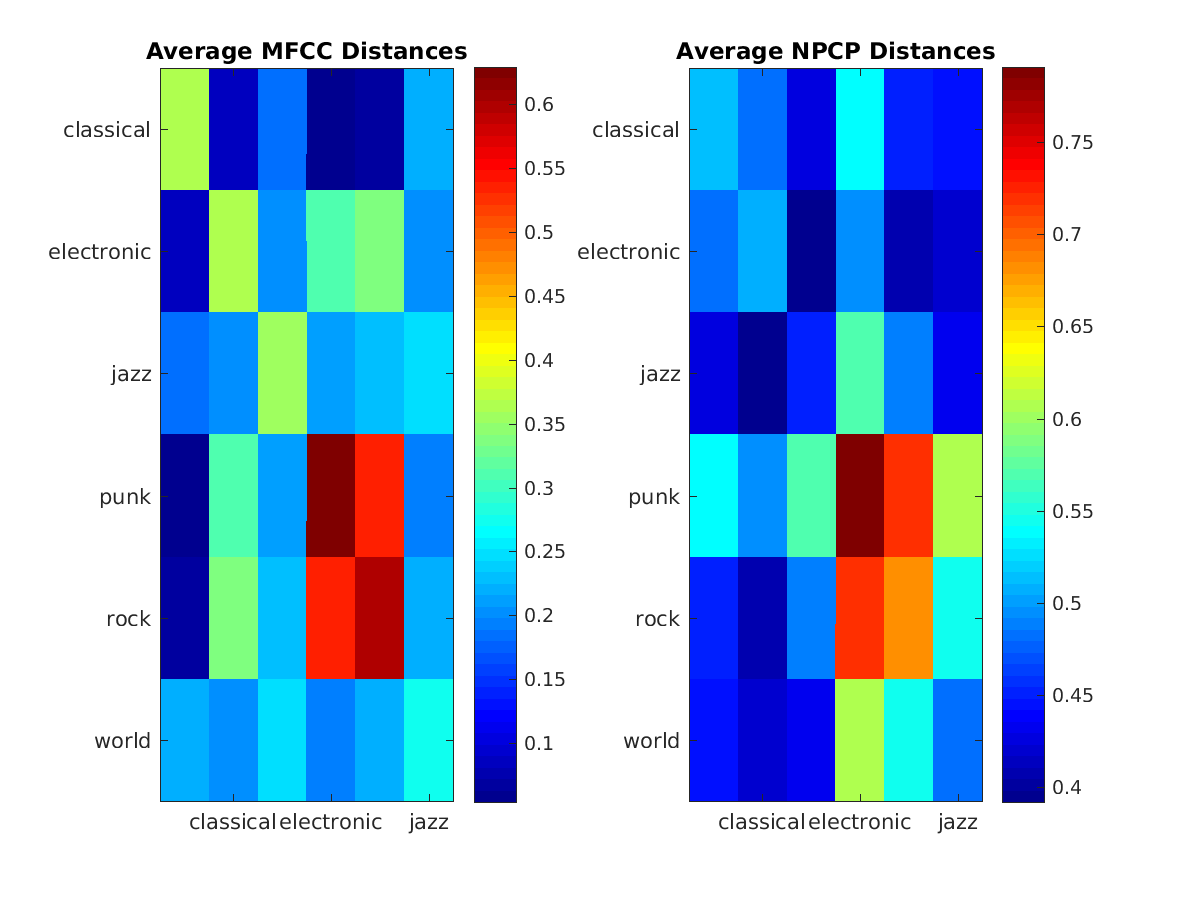
\includegraphics[width=1.25\textwidth]{length30.png}
    \caption{Song Length = 30}
\end{figure}


\begin{figure}[H]
\hspace*{-2cm}    
    \centering
    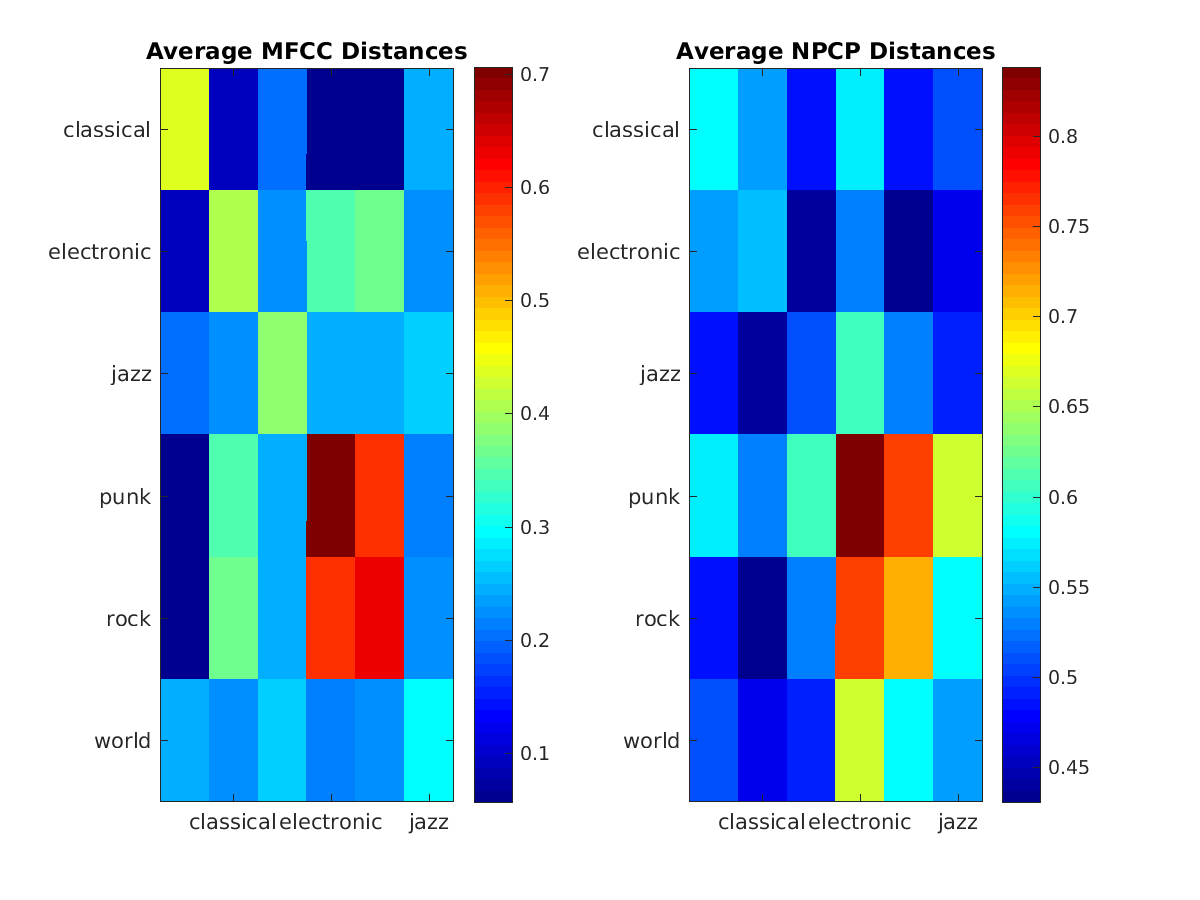
\includegraphics[width=1.25\textwidth]{length60.png}
    \caption{Song Length = 60}
\end{figure}


\begin{figure}[H]
\hspace*{-2cm}    
    \centering
    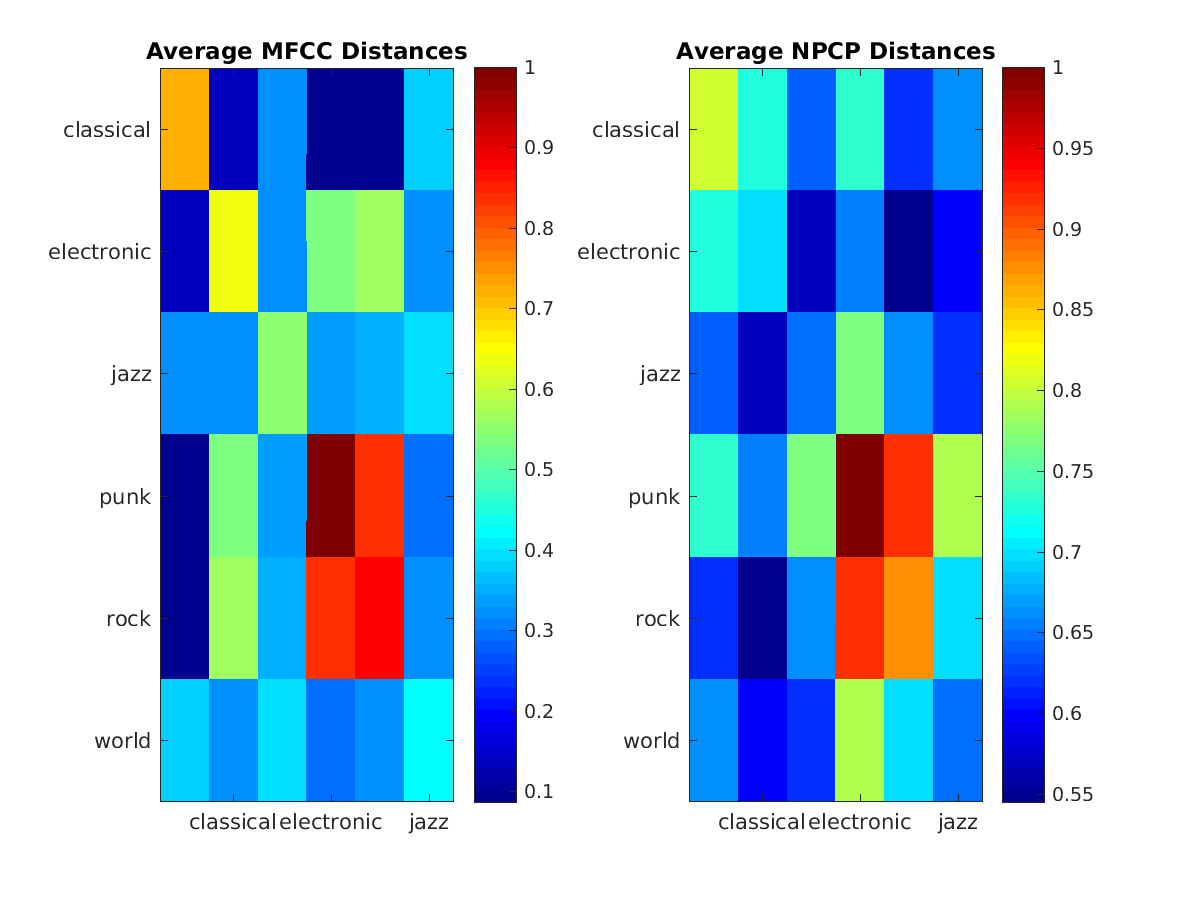
\includegraphics[width=1.25\textwidth]{average30.png}
    \caption{Song Length = 120}
\end{figure}


\begin{figure}[H]
\hspace*{-2cm}    
    \centering
    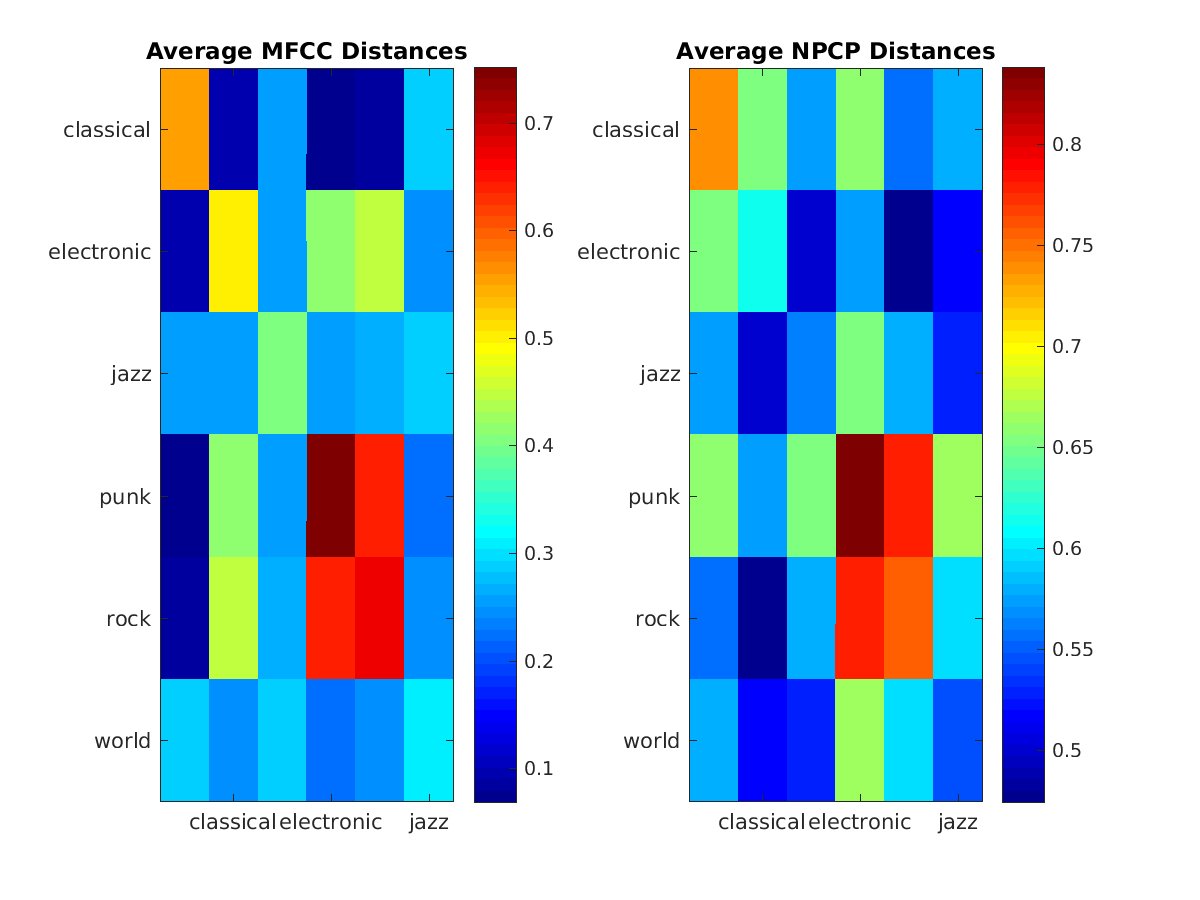
\includegraphics[width=1.25\textwidth]{length240.png}
    \caption{Song Length = 240}
\end{figure}

Overall, it seems that the length of song helps with the distance. This would make more sense because you obtain more song characteristics, but this can also be counterproductive because more characteristics may be too broad and not bring in enough specific details.


\section{Classification}

In order to test classification, there are two methods that are used: SVM and K Nearest Neighbor. The lab states that the SVM can be used to assist the original classifier, however, this is not necessarily possible to combine these two classifiers in Matlab. Instead, I will analyze the two different classifier methods. \\

\lstinputlisting[language=Matlab]{../classification.m}

	
\lstinputlisting[language=Matlab]{../genreClassifier.m}

\subsection{Confusion Matrices}

K Nearest Neighbor Averages \hfill $\left(\begin{array}{cccccc} 22.0 & 0 & 0.1 & 0 & 0 & 2.5\\ 0 & 17.0 & 2.4 & 1.5 & 1.6 & 2.4\\ 1.4 & 1.8 & 18.0 & 2.0 & 0 & 2.1\\ 0 & 1.5 & 0.9 & 18.0 & 3.1 & 1.5\\ 0 & 5.6 & 0.1 & 3.5 & 14.0 & 1.6\\ 4.4 & 3.5 & 3.2 & 0.7 & 0.9 & 12.0 \end{array}\right)
$ \\

SVM Averages \hfill
$\left(\begin{array}{cccccc} 22.0 & 0 & 0 & 0 & 0 & 3.3\\ 0 & 17.0 & 2.4 & 0.5 & 3.7 & 1.8\\ 0.1 & 2.3 & 14.0 & 2.0 & 0.1 & 6.2\\ 0 & 2.4 & 0 & 21.0 & 1.8 & 0\\ 0 & 4.2 & 0.4 & 4.2 & 14.0 & 2.6\\ 4.5 & 3.6 & 3.4 & 0.9 & 0.8 & 12.0 \end{array}\right)$

K Nearest Neighbor Standard Deviation \hfill $\left(\begin{array}{cccccc} 1.5 & 0 & 1.2 & 0 & 0 & 1.2\\ 0 & 2.3 & 1.6 & 1.3 & 0.85 & 1.4\\ 0.84 & 1.5 & 2.1 & 0.95 & 0.32 & 2.0\\ 0 & 1.3 & 0.7 & 2.0 & 1.2 & 0.63\\ 0 & 1.4 & 0.32 & 1.9 & 1.5 & 1.6\\ 2.3 & 1.9 & 1.8 & 0.32 & 0.79 & 2.5 \end{array}\right)
$

SVM Standard Deviation \hfill $\left(\begin{array}{cccccc} 3.1 & 0 & 0.42 & 0 & 0 & 2.9\\ 0 & 1.7 & 0.99 & 1.3 & 2.1 & 0.97\\ 1.0 & 1.6 & 1.6 & 1.4 & 0.67 & 1.5\\ 0 & 0.84 & 0.95 & 1.9 & 1.3 & 0\\ 0 & 2.3 & 0.79 & 1.6 & 1.9 & 0.95\\ 2.0 & 1.0 & 1.3 & 0.63 & 0.74 & 2.1 \end{array}\right)$

	
The values of the resulting confusion matrices demonstrates that the K nearest neighbor is the most efficient classifier overall. The values when compared to the histogram is as expected. The average mfcc images demonstrates how there are a lot of misclassification in the genres that were expected to have a lot of inconsistencies. The overall perentage of the KNN method is only 67.8\% and for SVM it is 65.8\%. There are a lot of misclassification between all the genres. This is strongly influenced by genres like world. For each genre, the accuracy is: 89\%, 68.4\%, 70.8\%, 72\%, 56.8\%, and 49.2\%. World, rock, and electronic give the classifier a much more difficult time to properly classify. 

\section{Conclusion}

The project was a great learning process and demonstrated different DSP techniques that can be applied in order to analyze audio. Just this single category demonstrates the power of filters and their use in the audio world. \\

It would be interesting to try and do a theoretical part of designing filters on our own and learning other types of techniques that are used to design these filter banks. \\

It would be interesting to be able to use two different representations to try and create a better distance matrix. The chroma was very lacking, as evident in the analysis of the distance matrices. Overall, this means that the chroma has some limitations in being able to represent different songs, most likely due to its limitations in representing different audio frequency ranges. \\

The classifier is a very difficult part of the project. In order to properly classify, it would require a lot more work to properly train and get working. 

\end{document}

